\documentclass[a4paper,12pt]{article}
\usepackage[top = 2.5cm, bottom = 2.5cm, left = 2.5cm, right = 2.5cm]{geometry}
\usepackage[T1]{fontenc}
\usepackage[utf8]{inputenc}
\usepackage{multirow} 
\usepackage{booktabs} 
\usepackage{graphicx}
\usepackage[spanish]{babel}
\usepackage{setspace}
\setlength{\parindent}{0in}
\usepackage{float}
\usepackage{fancyhdr}
\usepackage{amsmath}
\usepackage{amssymb}
\usepackage{amsthm}
\usepackage[numbers]{natbib}
\newcommand\Mycite[1]{%
	\citeauthor{#1}~[\citeyear{#1}]}
\usepackage{graphicx}
\usepackage{subcaption}
\usepackage{booktabs}
\usepackage{etoolbox}
\usepackage{minibox}
\usepackage{hyperref}
\usepackage{xcolor}
\usepackage[skins]{tcolorbox}
%---------------------------

\newtcolorbox{cajita}[1][]{
	 #1
}

\newenvironment{sol}
{\renewcommand\qedsymbol{$\square$}\begin{proof}[\textbf{Solución.}]}
	{\end{proof}}

\newenvironment{dem}
{\renewcommand\qedsymbol{$\blacksquare$}\begin{proof}[\textbf{Demostración.}]}
	{\end{proof}}

\newtheorem{problema}{Problema}
\newtheorem{definicion}{Definición}
\newtheorem{ejemplo}{Ejemplo}
\newtheorem{teorema}{Teorema}
\newtheorem{corolario}{Corolario}[teorema]
\newtheorem{lema}[teorema]{Lema}
\newtheorem{prop}{Proposición}
\newtheorem*{nota}{\textbf{NOTA}}
\renewcommand\qedsymbol{$\blacksquare$}
\usepackage{svg}
\usepackage{tikz}
\usepackage[framemethod=default]{mdframed}
\global\mdfdefinestyle{exampledefault}{%
linecolor=lightgray,linewidth=1pt,%
leftmargin=1cm,rightmargin=1cm,
}




\newenvironment{noter}[1]{%
\mdfsetup{%
frametitle={\tikz\node[fill=white,rectangle,inner sep=0pt,outer sep=0pt]{#1};},
frametitleaboveskip=-0.5\ht\strutbox,
frametitlealignment=\raggedright
}%
\begin{mdframed}[style=exampledefault]
}{\end{mdframed}}
\newcommand{\linea}{\noindent\rule{\textwidth}{3pt}}
\newcommand{\linita}{\noindent\rule{\textwidth}{1pt}}

\AtBeginEnvironment{align}{\setcounter{equation}{0}}
\pagestyle{fancy}

\fancyhf{}









%----------------------------------------------------------
\lhead{\footnotesize Álgebra Moderna}
\rhead{\footnotesize  Rudik Roberto Rompich}
\cfoot{\footnotesize \thepage}


%--------------------------

\begin{document}
 \thispagestyle{empty} 
    \begin{tabular}{p{15.5cm}}
    \begin{tabbing}
    \textbf{Universidad del Valle de Guatemala} \\
    Departamento de Matemática\\
    Licenciatura en Matemática Aplicada\\\\
   \textbf{Estudiante:} Rudik Roberto Rompich\\
   \textbf{Correo:}  \href{mailto:rom19857@uvg.edu.gt}{rom19857@uvg.edu.gt}\\
   \textbf{Carné:} 19857
    \end{tabbing}
    \begin{center}
        MM2035 - Álgebra Moderna - Catedrático: Ricardo Barrientos\\
        \today
    \end{center}\\
    \hline
    \\
    \end{tabular} 
    \vspace*{0.3cm} 
    \begin{center} 
    {\Large \bf  Tarea 13
} 
        \vspace{2mm}
    \end{center}
    \vspace{0.4cm}
%--------------------------
Problemas 1, 2, 3, 4, 5 y 6, sección 5.7.


\begin{problema}[Problema 1]
    If $p(x)$ is solvable by radicals over $F$, prove that we can find a sequence of fields
    $$
    F \subset F_1=F\left(\omega_1\right) \subset F_2=F_1\left(\omega_2\right) \subset \cdots \subset F_k=F_{k-1}\left(\omega_k\right),
    $$
    where $\omega_1^{r_1} \in F, \omega_2^{r_2} \in F_1, \ldots, \omega_k^{r_k} \in F_{k-1}, F_k$ containing all the roots of $p(x)$, such that $F_k$ is normal over $F$.
    \begin{dem}
        Esta deducción viene de un lema demostrado en clase, sea $f(x)$ soluble por radicales sobre $F\implies$ existe una cadena de campos $F=L_0\subseteq \cdots\subseteq L_s\ni L_i=L_{i-1}(\alpha_i)$ y $\alpha_i^{t_i}\in L_{i-1},t_1\in \mathbb{Z}^+\implies [L_1:L_{i-1}]\in \mathbb{Z}^+\implies$ por el teorema 5A, $[L_i=L_{i-1}(\alpha_i):F]\in\mathbb{Z}^+\implies$ por el teorema 3B/C/G, $\alpha_i$ es algebraico sobre $F\implies \exists f_(x)\in F[x]$, mónico, de grado mínimo e irreducible sobre $F\ni f_i(\alpha_i)=0\implies$ por el corolario 1 al lema 5.6, todas las raíces $f_i(x)$ son de multiplicidad 1 $\implies$ todas las raíces $f_i(x)$ son distintas. Entonces, sea $f(x)=\prod_{i=1}^sf_i(x)\in F[x]$, mónica. Sea $K$ el campo de descomposición de $f(x)$ sobre $F\implies$ por el teorema 5PK es una extensión normal de $F$ y $\alpha_1,\cdots,\alpha_s\in K\implies L_i=F(\alpha_1)\subseteq K\implies L_2=L_1(\alpha_2)\subseteq K\implies L_s=L_{s-1}(\alpha_s)\subseteq K$. Para asegurar la existencia de la cadena repetida de campos, procédase por inducción sobre $S$:
        \begin{itemize}
            \item Si $s=0\implies F=L_0=K$, cumple lo requerido. 
            \item Supóngase el teorema válido para todos los enteros menores a $s$. 
            \item Si $\delta_1,\cdots,\delta_m$ son todas las raíces de $f_1(x),\cdots,f_{s_4}(x)$ y $E=F(\delta_1,\cdots,\delta_n)\implies \alpha_1,\cdots,\alpha_s\in E\implies L_i=F(\alpha_i)\subseteq E\implies L_2=L_1(\alpha_2)\subseteq E\implies\cdots \implies L_{s-1}=L_{s-2}(\alpha_{s-1})\subseteq E$. De esto, $E=F(\delta_1,\cdots,\delta_m)$ es el campo de descomposición de $\prod_{i=1}^{s-1}f_i(x)$ sobre $F\implies$ por la hipótesis de inducción, existe una cadena de campo la requerida para $E$ y $F$. Sean $\gamma_1,\cdots,\gamma_{gr(f_s)}$ las raíces de $f_s(x)$ y supóngase sin perdida de generalidad que $\alpha_s=\gamma$. Nótese que 
            $K=F(\delta_1,\cdots,\delta_m,\gamma_1,\cdots,\gamma_{gr(f_s)})=F(\delta_1,\cdots,\delta_m)(\gamma_1,\cdots,\gamma_{gr(fs)})=E(\gamma_1,\cdots,\gamma_{gr(f_s)})$, por el teorema 5P, una extensión normal de $F\implies$ por el lema 5.9,$\exists \sigma_i\in G(K,F)\ni \sigma_i(\alpha_s)=\sigma_(\gamma_i)=\gamma_i\implies \sigma_i(\alpha_s^{t_s})=\sigma_i(\alpha_s)^{t_s}=\gamma_i^{t_s}$. Pero, $\alpha_s^{t_s}\in L_{s-1}\subseteq E$, una extensión normal de $F\implies E\subseteq K\implies$ por $(i)$ del Teorema Fundamental de la Teoría de Galois (5Q) $K_{G(K,E)}=E\implies \gamma_{t_s}=\sigma_i(\gamma_s^{t_s})=\gamma_s^{t_s}\in E\implies$ la cadena de campos que se obtiene (por hipótesis inductiva) con la cadena $E=E_0\subseteq E_1=E(\gamma_1)\subseteq E_2=E_1(\gamma_2)\subseteq \cdots \subseteq E_{gr(f_s)}=E_{gr(f_s)-1}(\gamma_{gr(f_s)})=K$, con $\gamma_i^{t_s}\in E\subseteq E_{i-1}$
        \end{itemize}
        
    \end{dem}
\end{problema}

\begin{problema}[Problema 2]
    Prove that a subgroup of a solvable group is solvable.
    \begin{dem}
        Sea $G$ un grupo soluble y sea $H$ un subgrupo de $G$ ($H\subseteq G$), por \textbf{lema 3.10} $\exists k\in\mathbb{N}\ni G^{(k)}=(e)$. A probar: $\exists k\in\mathbb{N}\ni H^{(k)}=(e)$.\bigbreak
        
        Usando la deducción del lema 3.10: Si $G^{(k)}=(e)$, sean $N_0=G, N_1=G^{\prime}, \cdots, N_i=G^i, \cdots, N_k=G^{(k)}=$ $(e) \Longrightarrow G=N_0 \supseteq G^{\prime} \supseteq \cdots \supseteq G^{(i)} \supseteq \cdots \supseteq G^{(k)}=(e), G^{(i)}$ es un subgrupo normal de $G^{(i-1)}$ y
        
        $$\frac{N_{i-1}}{N_i}=\frac{G^{i-1}}{G^{(i)}}$$ 
        es abeliano. Ahora bien, como $H\subseteq G$, supóngase que $H$ es normal, entonces las intersecciones $H\cap N_i$ y $H\cap N_{i-1}$ también son normales, se vuelve a aplicar el mismo argumento:
        
        $$\frac{H\cap N_{i-1}}{H\cap N_i}=\frac{H\cap G^{i-1}}{H\cap G^{(i)}}$$ 
        
        es abeliano. Por lo tanto $\exists k\in\mathbb{N}\ni H^{(k)}=(e)$, probando que un subgrupo de un grupo soluble es soluble.
    
    \end{dem}
\end{problema}

\begin{problema}[Problema 3]
    Prove that $S_4$ is a solvable group.
    \begin{dem}
        Para demostrar que $S_4$ es un grupo soluble, usaremos el algoritmo desarrollado en el lema 3.10. Para esto, considérese todos los subgrupos de orden $n$ de $S_4$, subclasificados por su clase de conjugación: 
        \begin{figure}[H]
            \centering
            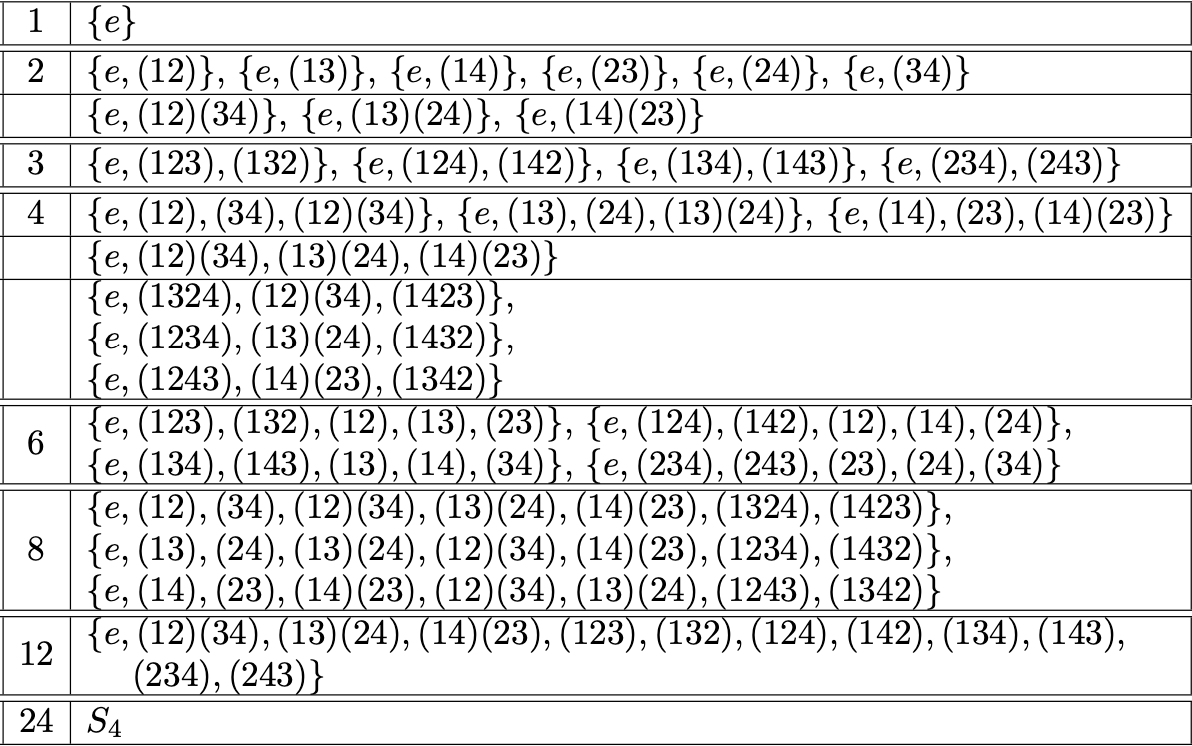
\includegraphics[scale=0.5]{Problemas/1.png}
        \end{figure}

        En donde, determinaremos los subgrupos normales, los cuales se definen como: un subgrupo es normal si es igual a todos los subgrupos conjugados (es decir, tiene un único elemento en su clase de conjungación). Considerando la tabla, se tiene la identidad, uno de las clases de conjugaciones de $A_4$, la única clase de $A_{12}$ y $S_4$. Por la forma en el algoritmo está planteado en el lema 3.10, tomaremos al subgrupo normal definido por la clase de conjugación $\{e,(12),(34),(13)(24),(14)(23)\}$. Entonces, sea 

        $$(e)\subseteq \{e,(12),(34),(13)(24),(14)(23)\}\subseteq A_4\subseteq S_4,$$
        Nótese que todas los conjuntos son normales, lo que nos permite concluir que 


        $$\frac{A_4}{\{e,(12),(34),(13)(24),(14)(23)\}}\quad\text{y}\quad \frac{S_4}{A_4}$$
        son abelianos. Por la definición de soluble, $S_4$ es un grupo soluble.

    \end{dem}
\end{problema}

\begin{problema}[Problema 4]
    If $G$ is a group, prove that all $G^{(k)}$ are normal subgroups of $G$.
    \begin{dem}
        Procedemos por inducción sobre $k$. 
        \begin{itemize}
            \item Paso base, si $k=1$, entonces: 
            $$G^{(1)}=\{x,y\in G|xyx^{-1}y^{-1}\},$$
            el cual es un subgrupo normal de $G$.
            \item Hipótesis inductiva, supóngase que todos los $G^{(i-1)}$ son subgrupos normales de $G$. 
            \item Paso inductivo, debemos probar que  todos los $G^{(i)}$ son subgrupos normales en $G$, sean $x,y\in G^{(i-1)}$ y $g\in G$. Por la hipótesis, $g(xyxy^{-1})g^{-1}\in G^{i-1}$, tal que por una de las caracterizaciones de los subgrupos normales:
            \begin{align*}
                g(xyxy^{-1})g^{-1} &= gxyxy^{-1}g^{-1}\\
                                         &= gx(gg^{-1})y(gg^{-1})x^{-1}(gg^{-1})y^{-1}g^{-1}\\
                                         &= gx(g^{-1}g)y(g^{-1}g)x^{-1}(g^{-1}g)y^{-1}g^{-1}\\
                                         &= g(x)g^{-1}g(y)g^{-1}g(x^{-1})g^{-1}g(y^{-1})g^{-1}\in G^{i}
            \end{align*}
            Entonces, todos los $G^{(i)}$ son subgrupos normales de $G$. 
        \end{itemize}
    \end{dem}
\end{problema}

\begin{problema}[Problema 5]
    If $N$ is a normal subgroup of $G$ prove that $N^{\prime}$ must also be a normal subgroup of $G$.
    \begin{dem}
        Sea $N$ un subgrupo normal de $G$, además sea $N'=\{a,b\in N|aba^{-1}b^{-1}\}$, además sea $\forall z\in N,\forall x\in G \ni zxz^{-1}\in N$. Sea entonces $x,y\in N\implies xyx^{-1}y^{-1}\in N'\implies \forall g\in G$, 
        \begin{align*}
            g(xyxy^{-1})g^{-1} &= gxyxy^{-1}g^{-1}\\
                                     &= gx(g^{-1}g)y(g^{-1}g)x^{-1}(g^{-1}g)y^{-1}g^{-1}\\
                                     &= g(x)g^{-1}g(y)g^{-1}g(x^{-1})g^{-1}g(y^{-1})g^{-1}\\
                                     &= (g(x)g^{-1})(g(y)g^{-1})(g(x^{-1})g^{-1})(g(y^{-1})g^{-1})\in N
        \end{align*}
        Entonces $N^{\prime}$ es un subgrupo normal de $G$
    \end{dem}
\end{problema}




%---------------------------
%\bibliographystyle{apa}
%\bibliography{referencias.bib}

\end{document}